\title{Final Exam for Algebra-Based Physics: Mechanics (PHYS135A)}
\author{Dr. Jordan Hanson - Whittier College Dept. of Physics and Astronomy}
\documentclass[10pt]{article}
\usepackage[a4paper, total={18cm, 27cm}]{geometry}
\usepackage{outlines}
\usepackage[sfdefault]{FiraSans}
\usepackage{graphicx}

\begin{document}
\maketitle
\small
\section{Equations and Constants}
Pythagorean theorem (magnitude of a vector): $|v| = \sqrt{v_x^2+v_y^2}$ \\
Dot-product of two vectors: $\vec{u} \cdot \vec{v} = uv\cos\theta = u_x v_x + u_y v_y$ \\
Displacement: $\Delta \vec{x} = \vec{x}_f - \vec{x}_i$ \\
Average velocity: $\vec{v} = \Delta \vec{x}/\Delta t$ \\
Average acceleration: $\vec{a} = \Delta \vec{v}/\Delta t$ \\
Kinematic equation 1 (constant acceleration): $v(t) = v_i + at$ \\
Kinematic equation 2 (constant acceleration): $x(t) = \frac{1}{2}at^2+v_i t+x_i$ \\
Kinematic equation 3 (constant acceleration): $v_f^2 = v_i^2 + 2 a \Delta x$ \\
Newton's First Law: if $\vec{F}_{Net} = 0$, $\vec{v} = const$ (or zero) \\
Newton's Second Law: $\vec{F}_{Net} = m \vec{a}$ \\
Newton's Third Law: $\vec{F}_{AB} = - \vec{F}_{BA}$ \\
Weight force: $\vec{w} = -mg\hat{j}$ \\
Normal force: $\vec{N} = +mg\hat{j}$ (unless surface is not flat) \\
Force of friction: $\vec{f}_f = -\mu \vec{N}$ \\
Spring force: $F_s = -k\Delta \vec{x}$ \\
Drag force: $F_D = \frac{1}{2}C\rho A v^2$ \\
Definition of the radian: $s = r \theta$ \\
Angular velocity (change in radians per unit time): $\omega = \Delta \theta/\Delta t$ \\
Angular velocity (change in $\omega$ per unit time): $\alpha = \Delta \omega/\Delta t$ \\
Tangential velocity: $v = r\omega$ \\
Tangential acceleration $a = r\alpha$ \\
Centripetal acceleration: $a_c = r\omega^2 = v^2/r$ \\
Centripetal force: $F_c = m a_c$ \\
Newton's Law of Gravity: $F_G = G m_1 m_2 / r^2$, $G = 6.674\times 10^{-11}$ N m$^2$ kg$^{-2}$ \\
Kepler's 3rd Law (explicit): $r^3/T^2 = \frac{G}{4\pi^2} M$, where $M$ is the mass of the central body. \\
Kepler's 3rd Law (scaling): $r_1^3/T_1^2 = r_2^3/T_2^2 = const$ \\
Definition of Work: $W = \vec{F} \cdot \vec{d} = Fd\cos\theta$ \\
Definition of kinetic energy: $KE = \frac{1}{2} mv^2$ \\
Work-Energy theorem: $W = \Delta KE$ \\
Definition of gravitation potential energy: $U = mgh$ \\
Conservation of energy: $KE_i + U_i = KE_f + U_f$ \\
Conservation of momentum: $\vec{p}_{i,1} + \vec{p}_{i,2} = \vec{p}_{f,1} + \vec{p}_{f,2}$ \\
\textit{Definition: elastic collision}. Kinetic energy is conserved, along with momentum. \\
\textit{Definition: inelastic collision}. Kinetic energy is not conserved, but momentum is. \\

\section{Vectors}
\begin{enumerate}
\item Consider Fig. \ref{fig:tri}.  (a) If $a=3$ km, and $b=4$ km, what is $c$? (b) Imagine the line segment AB represents a vector $\vec{d}$.  What angle is between $\vec{d}$ and the horizontal axis? (What is the lower-left angle in the triangle)?
\begin{figure}[hb]
\centering
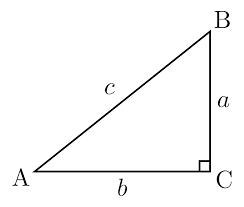
\includegraphics[width=0.25\textwidth]{figures/tri.png}
\caption{\label{fig:tri} A right triangle with side lengths of $a$ and $b$, and a hypoteneuse of $c$.}
\end{figure}
\end{enumerate}
\section{Kinematics}
\begin{enumerate}
\item We are tracking a drone through Whittier College.  The drone begins on top of the Science and Learning Center (SLC), at a height of 40 m.  It proceeds North towards Platner Hall, traveling 150 m in 10 seconds.  Next, it proceeds Northwest for 117 m, and arrives at the flagpole on the North Lawn 8 seconds later. Finally, it heads South for 220 m, reaching Villalobos Hall in 12 seconds.  (a) What is the velocity of the first line-segment of the flight?  (b) What is the velocity of the second line-segment of the flight? (c) What is the velocity of the third line-segment of the flight?  (d) What is the total distance traveled? (e) What is the total displacement? \textit{Hint: draw a coordinate system with the origin as the starting point.} \\ \vspace{2.5cm}
\item Suppose basketball player is shooting a free-throw.  The ball is at a horizontal distance of 5.8 m from the hoop.  The ball starts at the player's shoulder, 2.0 m above the ground.  The hoop is 3.0 m above the ground.  The shot goes in 1.25 seconds after the player shoots.  (a) Draw a diagram of the ball's trajectory. (b) What is the horizontal speed of the ball? (c) What is the vertical displacement of the ball at the moment it goes in the hoop? (d) What is the vertical speed of the ball when it is launched by the player? \\ \vspace{2.0cm}
\end{enumerate}
\section{Newton's Laws and Various Forces}
\begin{enumerate}
\item (a) What is the net force applied on the tooth in Fig. \ref{fig:mouth} if the tension in the wire is 25.0 N?  (b) Suppose the gum applies a force of 12 N in the positive y-axis.  What is the net force on the tooth?
\begin{figure}[hb]
\centering
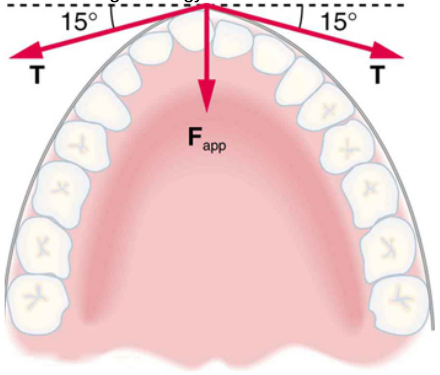
\includegraphics[width=0.25\textwidth]{figures/mouth.png}
\caption{\label{fig:mouth} Braces apply a net force on a tooth.}
\end{figure} \\
\item Consider an object on an inclined surface, held in a fixed position by static friction. (a) Draw the free-body diagram, including all relevant forces.  (b) Show that $\mu_s = \tan\theta$.  (c) If $\theta=20^{\circ}$, what is $\mu_s$? (c) We tilt the incline until the object begins to accelerate down the incline.  Draw the new free-body diagram. (d) Show that the acceleration is given by $a = g(\sin\theta-\mu_k \cos\theta)$.  (e) If $\theta=25^{\circ}$ and $a=0.1$ m/s$^2$, what is $\mu_k$? \\ \vspace{2.5cm}
\item A meteorite is flying through space at constant velocity, but then accelerates because it is pulled towards the Earth by gravity.  When it enters the atmosphere it reaches \textit{terminal velocity} before it burns up. (a) Sketch a curve that describes the velocity versus time of the meteorite.  (b) Assume the drag coefficient and area of the object are $C=0.5$ and $A=4$ m$^2$, and that $\rho_{air} = 1.225$ kg/m$^3$.  What is the drag force on the meteorite if it's traveling at 100 m/s? (c) Setting the drag force equal to the weight $mg$ yields the \textit{terminal velocity} $v_{T}$.  What is $v_{T}$ for the meteorite if it has a mass of 8000 kg? \\ \vspace{3cm}
\end{enumerate}
\section{Rotational Motion and The Law of Gravity}
\begin{enumerate}
\item Assume that Earth has an orbital period of 1.0 year, and an orbital radius of 1.0 AU.  The orbital period of Saturn is observed to be about 29 years.  How far from the Sun is Saturn (in AU)? (b) The orbital radius of Mars is about 1.5 AU.  What is the duration of the orbit of Mars, in years? \\ \vspace{1.5 cm}
\item A polisher in a machine shop is a rough wheel that spins, grinding surfaces until they are smooth.  (a) If the wheel turns at 360 rpm, and has a radius of 5 cm, what is the tangential velocity at the surface of the wheel? (\textit{Be careful with units}). (b) If the angular velocity of the wheel is accelerated from 360 to 720 rpm in 1.0 second, what is the angular acceleration? \\ \vspace{1.0cm}
\end{enumerate}
\section{Work, Energy and Momentum}
\begin{enumerate}
\item Consider Fig. \ref{fig:work}.  (a) Is work being done in either situation?  Explain why or why not in your own words. (b) Suppose the man lifts the briefcase against gravity, through a distance of 1.0 m.  If the briefcase weighs 1.5 kg, how much work has the man done? (c) If he drops the briefcase from a height of 2.0 m, what will be the final kinetic energy and velocity?
\begin{figure}[hb]
\centering
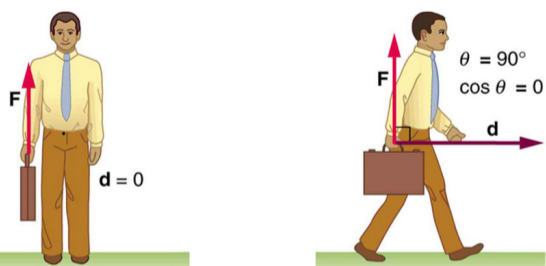
\includegraphics[width=0.5\textwidth]{figures/final1.png}
\caption{\label{fig:work} Two different scenarios regarding physical work.}
\end{figure}
\item Suppose an asteroid ejects a chunk of itself, changing the course of the main asteroid.  Let the mass of the initial object be $M$.  Let the small chunk after the separation have a mass $m_1$, and the new mass of the main asteroid be $m_2$.  Assume that we are moving alongside the main asteroid before the separation, such that we observe the velocity to be zero.  Let the velocity of the small chunk be $v_1'$ and that of the main asteroid be $v_2'$. (a) Using momentum conservation, show that the speed of the main asteroid after the separation is $v_2' = \left(\frac{m_1}{m_2}\right) v_1'$. (b) If we observe $v_1' = 100$ m/s, and $v_2' = 1$ m/s, and estimate that $m_1 = 1000$ kg, what is $m_2$?
\end{enumerate}
\end{document}